\section{Experimentos Computacionais}\label{sec:experimentos} 
Os experimentos computacionais foram executados em uma máquina Intel Dual-Core de 2.81 GHz de clock e
2GB de memória RAM, rodando o sistema operacional Linux. Os algoritmos das seções \ref{sec:faster}, \ref{sec:floydwarshall}, \ref{sec:johnson_queue}, \ref{sec:johnson_vector} e \ref{sec:bfs} foram implementados na 
linguagem de programação c e compilados com o compilador gcc na versão 4.8.2. A tabela \ref{table:algoritmos} apresenta esses cinco algoritmos. Na coluna 1 está o nome que o algoritmo vai assumir aqui, a coluna 2 é a referência da seção que o algoritmo foi apresentado,
a coluna 3 mostra o nome do arquivo de especificações do algoritmo e a coluna 4 apresenta o nome do arquivo com o código fonte do 
algoritmo.

\begin{table}[htbp]
\begin{center}
  \begin{tabular}{|c|c|c|c|}
    \hline
      Algoritmo                & Seção                    & Arquivo .h              & Arquivo .c            \\ \hline
      kc\_faster               & \ref{sec:faster}         & repeated\_squaring.h    & repeated\_squaring.c  \\ \hline
      kc\_floydwarshall        & \ref{sec:floydwarshall}  & floyd\_warshall.h       & floyd\_warshall.c     \\ \hline
      kc\_johnson\_min\_queue    & \ref{sec:johnson_queue}  & johnson.h               & johnson.c           \\ \hline
      kc\_johnson\_array        & \ref{sec:johnson_vector} & johnson.h               & johnson.c            \\ \hline
      kc\_nbfs                 & \ref{sec:bfs}            & bfs.h                   & bfs.c                 \\ \hline
  \end{tabular}
\caption{Algoritmos exatos para o problema de encontradar k comunidades em um grafo não direcionado e não ponderado}
\label{table:algoritmos}
\end{center}
\end{table}

Foram utilizados cinco conjuntos de instâncias de testes nos experimentos computacionais, três dessas instâncias foram retiradas de \cite{files_test} e as outras duas foram geradas por esse trabalho. As instâncias de teste retiradas de \cite{files_test}
foram: karate, lesmis e adjnoun. A instância karate representa uma rede social de 34 membros de um clube de karate, a instância
lesmis representa o número de ocorrências de determinados caracteres em um livro e a instância adjnoun representa
o número de ocorrências de palavras em um livro. As instâncias geradas vão ser chamadas de path e completo. Essas instâncias
foram geradas pois vão explorar o melhor e o pior caso dos algoritmos apresentados. Uma instância
path é um grafo onde o nó $i \in V$ está ligado ao nó $i+1 \in V$ formando apenas um caminho simples. Foram gerados três 
instâncias path com 50, 100 e 200 nós.  Uma instância completo é um grafo completo, ou seja, existe uma aresta
entre cada par de nós do grafo. Foram geradas três instâncias completo com 50, 100 e 200 nós.
A tabela \ref{table:instancias} apresenta todas as instâncias de teste. Na coluna 1 dessa tabela está o nome da instância,
a coluna 2 apresenta o número de nós da instância e a coluna 3 mostra o número de aresta de cada instância.

\begin{table}[htbp]
\begin{center}
  \begin{tabular}{|c|c|c|}
    \hline
      Instância                & \# Nós                   & \# Arestas \\ \hline
      karate                   & 34                       & 78 \\ \hline
      lesmis                   & 77                       & 254 \\ \hline
      adjnoun                  & 112                      & 425 \\ \hline
      path\_50                 & 50                       & 49 \\ \hline
      path\_100                & 100                      & 99 \\ \hline
      path\_200                & 200                      & 199 \\ \hline
      completo\_50             & 50                       & 2450 \\ \hline
      completo\_100            & 100                      & 9900 \\ \hline
      completo\_200            & 200                      & 39800 \\ \hline
  \end{tabular}
\caption{Características das instâncias de testes}
\label{table:instancias}
\end{center}
\end{table}

No primeiro experimento foi comparado a performance dos algoritmos das seções \ref{sec:faster}, \ref{sec:floydwarshall}, \ref{sec:johnson_queue}, \ref{sec:johnson_vector} e \ref{sec:bfs} nas instâncias retiradas de \cite{files_test}.
A figura \ref{karate} mostra os resultados obtidos com a execução dos algoritmos para a instância karate. Essa figura mostra
que o algoritmo mais rápido foi o de kc\_nbfs seguido do kc\_floydwarshall, essa figura também mostra que a medida
que o número de comunidades aumenta o algoritmo kc\_faster passa a ser o mais lento. O algoritmo kc\_johnson\_min\_queue
passa a ser mais rápido que o algoritmo kc\_johnson\_array com o aumento do número de comunidades.

\begin{figure}
\centering
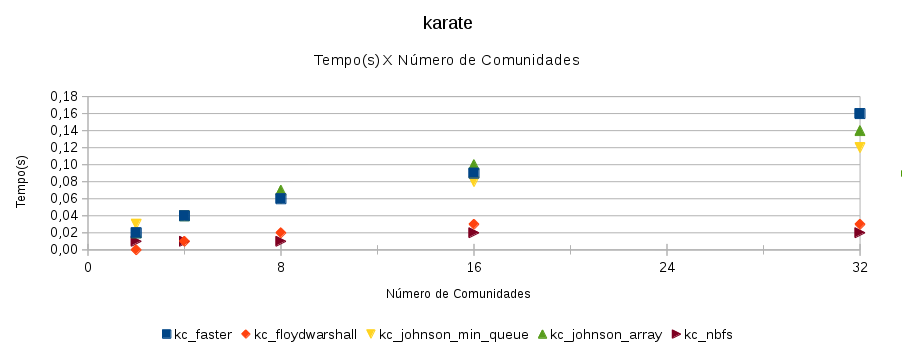
\includegraphics[width=6in]{karate.png}
\caption{Comparação de tempo em segundos pelo número de comunidades:2, 4, 8, 16 e 32 para os cinco algoritmos apresentados nas seções \ref{sec:faster}, \ref{sec:floydwarshall}, \ref{sec:johnson_queue}, \ref{sec:johnson_vector} e \ref{sec:bfs} e excutado na instância de teste karate}
\label{karate}
\end{figure}

A figura \ref{lesmis} mostra os resultados obtidos com a execução dos algoritmos para a instância lesmis. Essa figura mostra
que o algoritmo mais rápido foi o de kc\_nbfs seguido do kc\_floydwarshall, essa figura também mostra que a medida
que o número de comunidades aumenta o algoritmo kc\_faster passa a ser o mais lento. O algoritmo kc\_johnson\_min\_queue
passa a ser mais rápido que o algoritmo kc\_johnson\_array com o aumento do número de comunidades.

\begin{figure}
\centering
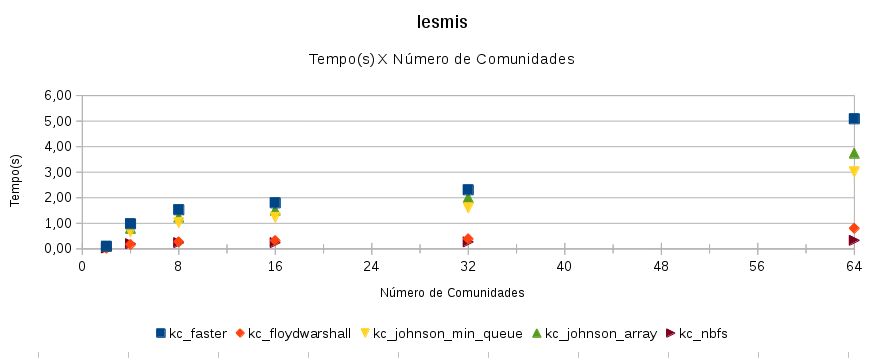
\includegraphics[width=6in]{lesmis.png}
\caption{Comparação de tempo em segundos pelo número de comunidades:2, 4, 8, 16, 32 e 64 para os cinco algoritmos apresentados nas seções \ref{sec:faster}, \ref{sec:floydwarshall}, \ref{sec:johnson_queue}, \ref{sec:johnson_vector} e \ref{sec:bfs} e excutado na instância de teste lesmis}
\label{lesmis}
\end{figure}

A figura \ref{adjnoun} mostra os resultados obtidos com a execução dos algoritmos para a instância adjnoun. Essa figura mostra
que o algoritmo mais rápido foi o de kc\_nbfs seguido do kc\_floydwarshall, essa figura também mostra que a medida
que o número de comunidades aumenta o algoritmo kc\_faster passa a ser o mais lento. O algoritmo kc\_johnson\_min\_queue
passa a ser mais rápido que o algoritmo kc\_johnson\_array com o aumento do número de comunidades.

\begin{figure}
\centering
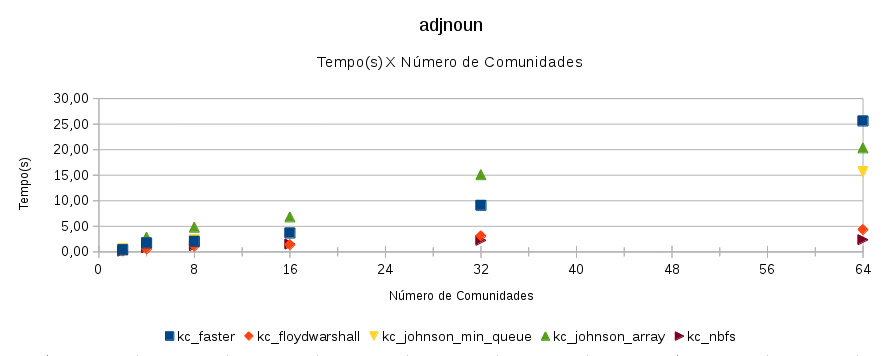
\includegraphics[width=6in]{adjnoun.png}
\caption{Comparação de tempo em segundos pelo número de comunidades:2, 4, 8, 16, 32 e 64 para os cinco algoritmos apresentados nas seções \ref{sec:faster}, \ref{sec:floydwarshall}, \ref{sec:johnson_queue}, \ref{sec:johnson_vector} e \ref{sec:bfs} e excutado na instância de teste adjnoun}
\label{adjnoun}
\end{figure}

No segundo experimento foi comparado a performance dos algoritmos das seções \ref{sec:faster}, \ref{sec:floydwarshall}, \ref{sec:johnson_queue}, \ref{sec:johnson_vector} e \ref{sec:bfs} no melhor e pior caso. No melhor caso, os algoritmos foram
executados nas instâncias path50, path100 e path200 com o número de comunidades $k$ igual a 50, 100 e 200 respectivamente, assim
todas as $k - 1$ arestas do grafo precisaram ser retiradas. No pior caso, os algoritmos foram executados nas instâncias completo50, completo100 e completo200 com número de comunidades $k$ igual a 50, 100 e 200 respectivamente, obrigando a
retirada de todas as arestas do grafo. Para comparar os algoritmos, o tempo de execução de cada um foi dividido pelo tempo 
de execução do algoritmo kc\_nbfs que foi o algoritmo que obteve o menor tempo de resposta.
A figura \ref{path} apresenta os resultados obtidos para as instâncias path50, path100 e path200.  Nessa figura o eixo
vertical representa o tempo que o algoritmo gastou dividido pelo tempo gasto pelo algoritmo kc\_nbfs e o eixo horizontal
representa cada uma das instâncias path. Obervando essa figura vemos que o algoritmo kc\_faster é o algoritmo que apresenta os piores resultados e com o aumento do número de arestas no grafo path a razão do tempo gasto por esse algoritmo e o algoritmo kc\_nbfs aumenta muito. O algoritmo kc\_floydwarshall consumiu tempos similares aos tempos do algoritmo kc\_nbfs. O algoritmo
kc\_johnson\_min\_queue foi mais rápido do que o algoritmo kc\_johnson\_array.

\begin{figure}
\centering
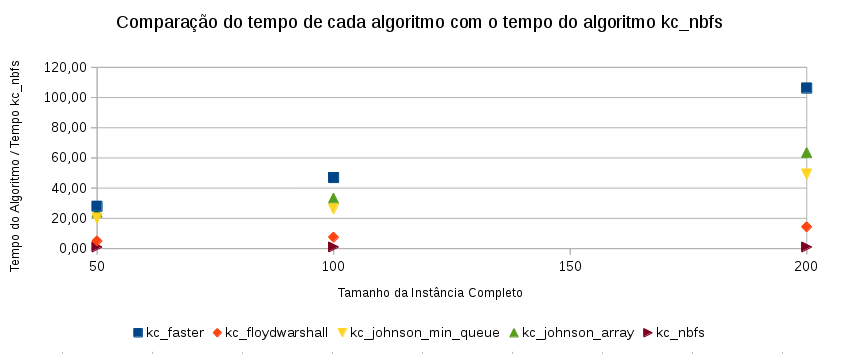
\includegraphics[width=6in]{path.png}
\caption{Comparação da razão do tempo gasto dos algoritmos pelo tempo gasto pelo algoritmo mais rápido nas instâncias path50, path100 e path200}
\label{path}
\end{figure}

A figura \ref{completo} apresenta os resultados obtidos para as instâncias completo50, completo100 e completo200.  Nessa figura o eixo vertical representa o tempo que o algoritmo gastou dividido pelo tempo gasto pelo algoritmo kc\_nbfs e o eixo horizontal
representa cada uma das instâncias completo. Obervando essa figura vemos que o algoritmo kc\_faster é o algoritmo que apresenta os piores resultados e com o aumento do número de arestas no grafo completo a razão do tempo gasto por esse algoritmo e o algoritmo kc\_nbfs aumenta muito. O algoritmo kc\_floydwarshall consumiu tempos similares aos tempos do algoritmo kc\_nbfs. O algoritmo
kc\_johnson\_min\_queue foi mais rápido do que o algoritmo kc\_johnson\_array.

\begin{figure}
\centering
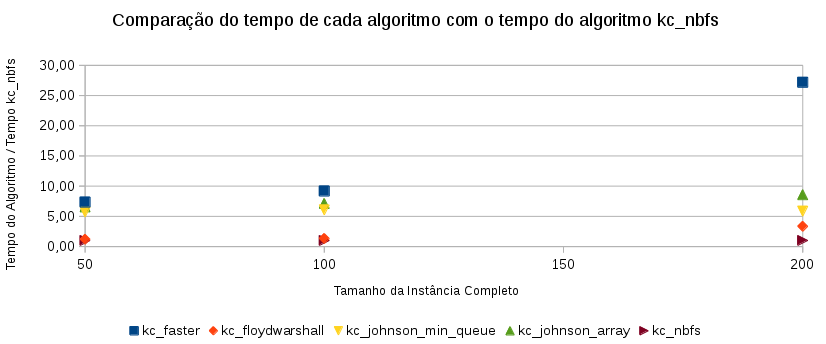
\includegraphics[width=6in]{completo.png}
\caption{Comparação da razão do tempo gasto dos algoritmos pelo tempo gasto pelo algoritmo mais rápido nas instâncias completo50,
completo100 e completo200}
\label{completo}
\end{figure}

Comparando as figuras \ref{path} e \ref{completo} a razão entre o tempo dos algoritmos e o tempo do algoritmo kc\_nbfs diminui, isso pode ser explicado porque com o aumento do número de arestas no grafo o algoritmo kc\_nbfs tende a ser muito pior.










